\subsection{MVC} 
\stefan{en smule malplaceret?}
MVC, or Model-View-Controller\cite{aspmvc}, is used to separate responsibility of an application into three parts; the model, the view, and the controller.
A diagram, displaying the pattern and its internal dependencies, can be seen in \Cref{mvcdiagram}.

\begin{figure}[h]
\begin{center}
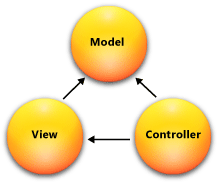
\includegraphics[width=\textwidth, trim={-4cm 11cm 5cm 1cm}]{mvc.pdf}
\caption{The MVC design pattern.}
\label{mvcdiagram}
\end{center}
\end{figure}\bruno{Meget bedre med den figur! Men måske større cirkler og større skrift :)}

\paragraph{Model} contains the model of the application domain and takes care of fetching data and making it available through the model.

In the case of our web service, the model is making resources available for the view.

\paragraph{View} displays the model to the user.
In our case the view is the serialized resource representation, that the user obtains by performing requests against the API.
Per default, this is \texttt{text/xml}, however, by adding the \texttt{Accept} header\cite[Section 14]{http_specification}, this can be set to \texttt{application/json}.

\paragraph{Controller} handles the interaction with users.
Based on user input, the controller works on the model and selects what the view needs to be used for displaying the data.

The routing to controllers is handled by the attributes \texttt{[RoutePrefix]} and \texttt{[Route]}.
In order to handle the different HTTP methods, controller methods are also annotated with an appropriate \texttt{[Http\{Method\}]} attribute (e.g. \texttt{[HttpGet]}) \cite{asp_routing}.